\documentclass[12pt, a4paper]{article}
\usepackage{graphicx}
\usepackage{xurl}
\usepackage{geometry}
\usepackage{float}
\usepackage{indentfirst}
\usepackage{amsmath}
% \usepackage{xcolor}
\usepackage[dvipsnames]{xcolor}


\geometry{left=2.54cm, right=2.54cm, top=3.18cm, bottom=3.18cm}
% \setlength{\parindent}{0pt}

\title{Hebbian Learning on Multilayer FNN}
\author{Liam (Min Goo)}

\begin{document}

\maketitle

\section*{~ 04/26}

\subsection*{Main Points}
\noindent
\begin{itemize}

    \begin{figure}
        \centering
        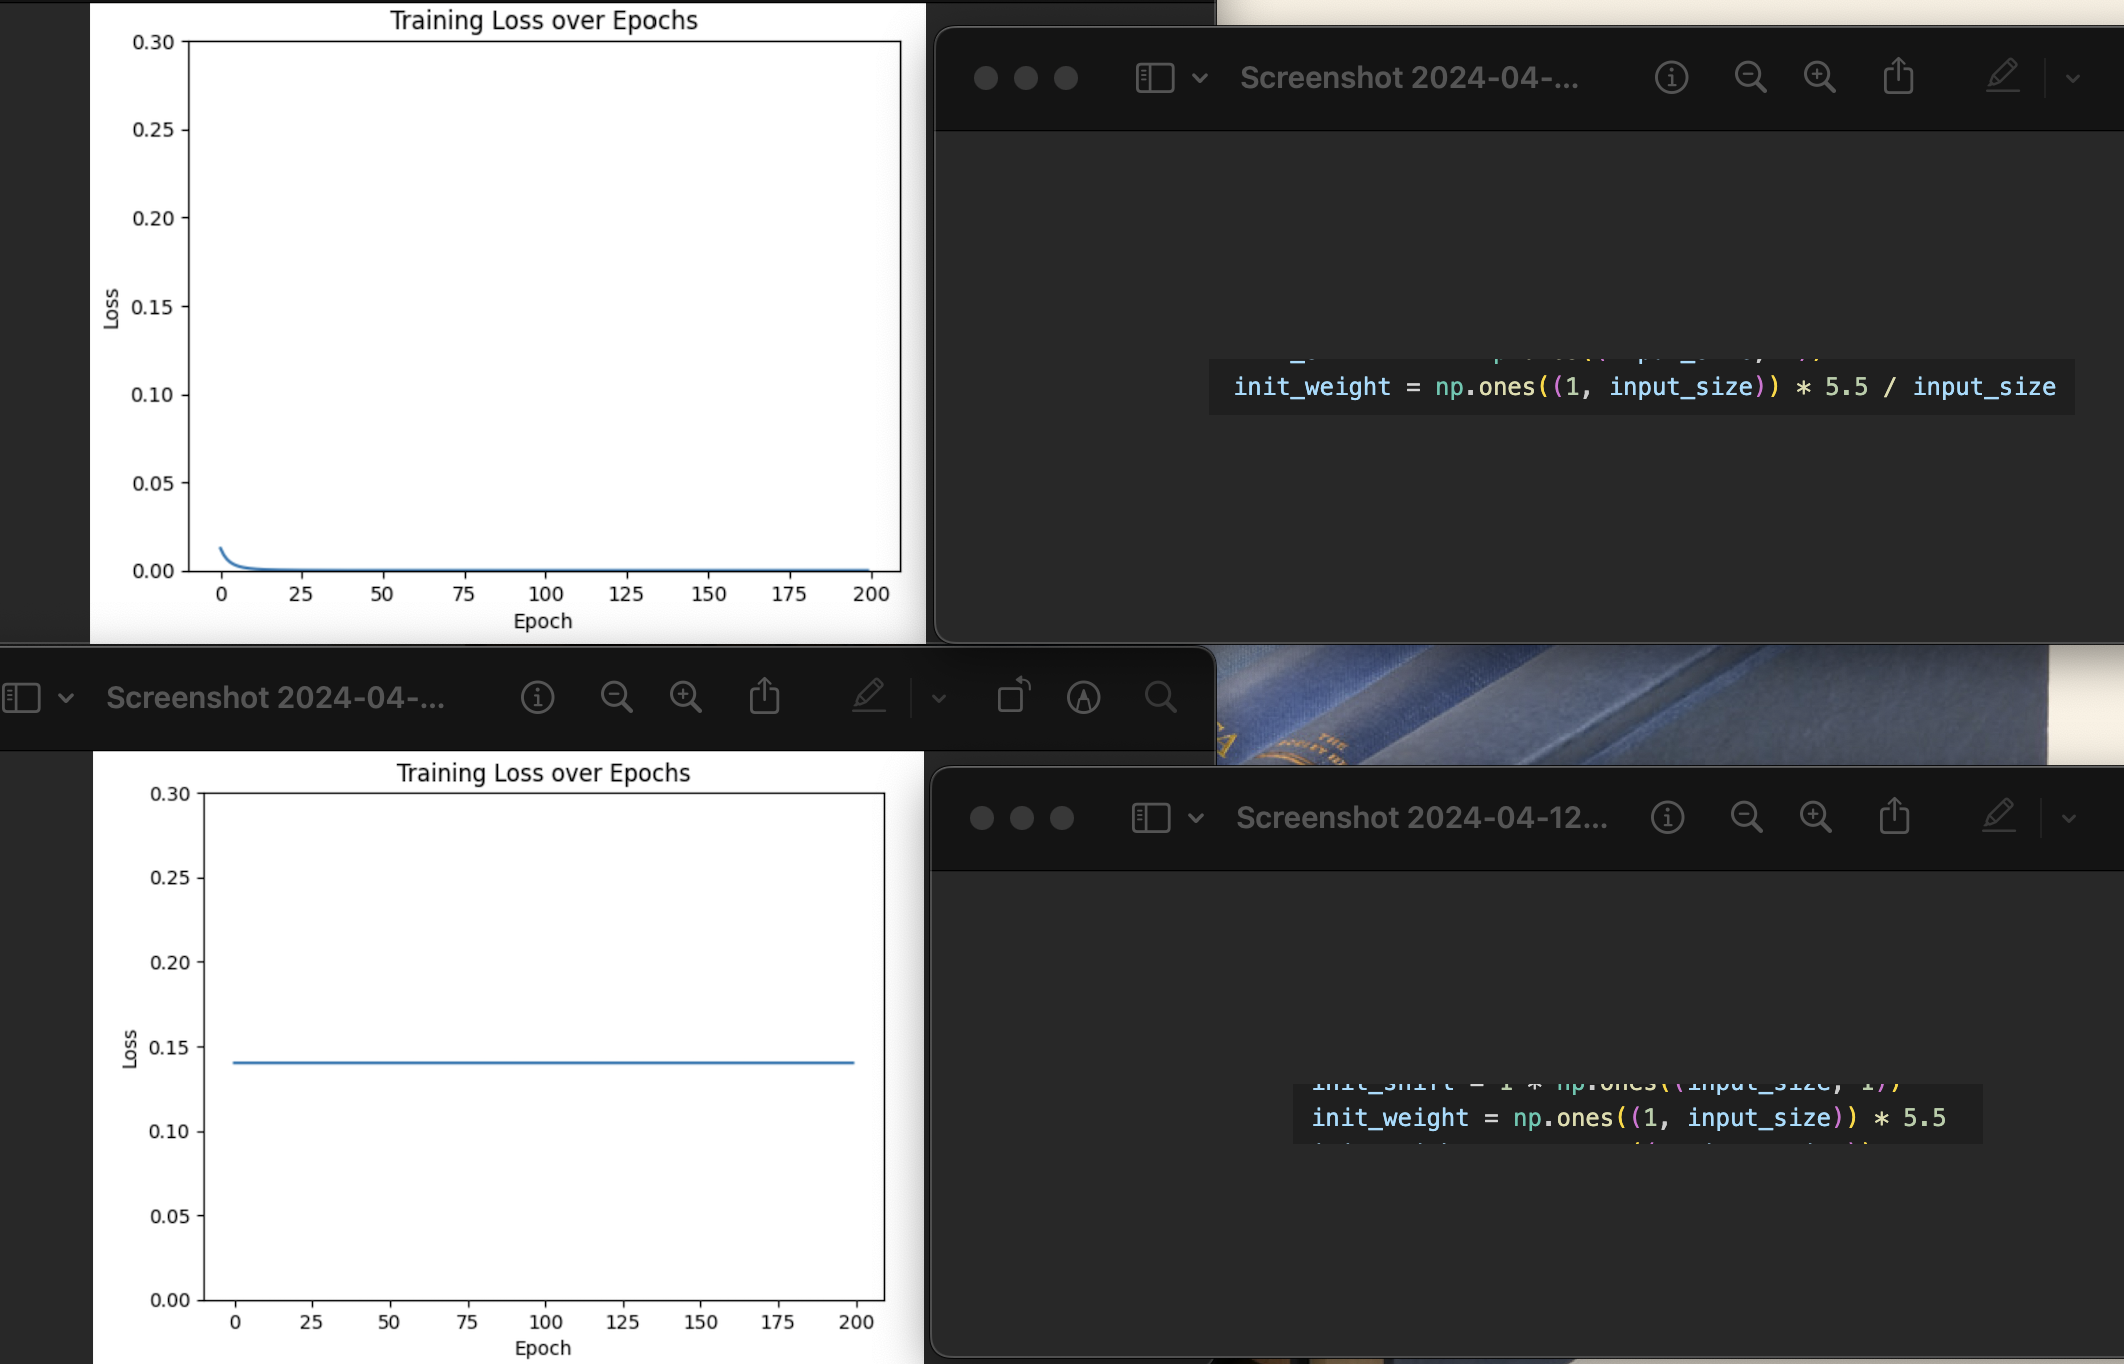
\includegraphics[width=0.5\linewidth]{training_loss_normalization.png}
        \caption{Loss change depending on normalization constant}
        \label{fig:enter-label}
    \end{figure}

    \item Original Plan: \textcolor{blue}{Fix function gradient failure} + \textcolor{red}{Test other complex functions and try classification}
    \item Fixed (partially): There was an issue where the hidden layer was not being updated while the first layer was, which turned out to be an implementation issue (has to do with current implementation creating a model for each iteration vs. conventionally only updating the variables). Jerry helped fixed this issue.
    \item Current problem: Hidden layer nodes are changing over time, but the \textcolor{red}{input node values do not change}. Despite no change in the initial layer there is a decrease in loss after a few epochs. Attempted to increase number of nodes to see if this would change initial nodes, but did not change. Implementation fix stage is taking much longer than expected.
    \item Plan: While debugging, I found out that normalization constant plays a key role in allowing gradient to happen. Dividing the initial values by input size determined whether the gradient occurred or not. I am planning to investigate whether this is the issue for the initial nodes as well.
    
\end{itemize}

\section*{~ 04/12}

\subsection*{Main Points}

\noindent
\begin{itemize}
    \item Original Plan: \textcolor{blue}{Fix data output} + \textcolor{red}{Implement Hebbian learning on Multilayer FNN}
        % \subitem \item \color{RubineRed}{Fix minor data + Implement Hebbian learning on Multilayer FNN}
    \item Current problem: \color{ForestGreen}{constant loss for Multilayer FNN}\color{black}
    \item While Single Layer FNN loss decreases over epoch, current multilayer model has constant loss
        \subitem attempts:
        \subitem 1 - different values for gains/shifts
        \subitem 2 - different values for weights
        \subitem 3 - hyperparameters (learning rate + momentum)
        \subitem (Single Layer FNN has 230 inputs with \textbf{same} initial gain/shift/weight values)
    \item given that a single layer with 230 inputs work, it seems the problem isn't computational, given that current multilayer  fails to decrease loss even for 20 inputs with 10 hidden-layer nodes
    \item future attempts
        \subitem 4 - feeding it to gaussian function prior to hidden layer?
            \subitem current: input $\rightarrow$ gaussian $\rightarrow$ hidden $\rightarrow$ weight $\rightarrow$ output
            \subitem attempt: input $\rightarrow$ gaussian $\rightarrow$ hidden \color{red} $\rightarrow$ gaussian \color{black} $\rightarrow$ weight $\rightarrow$ output
        \subitem 5 - implementing SGD optimizer from scratch
        
    \begin{figure}
        \centering
        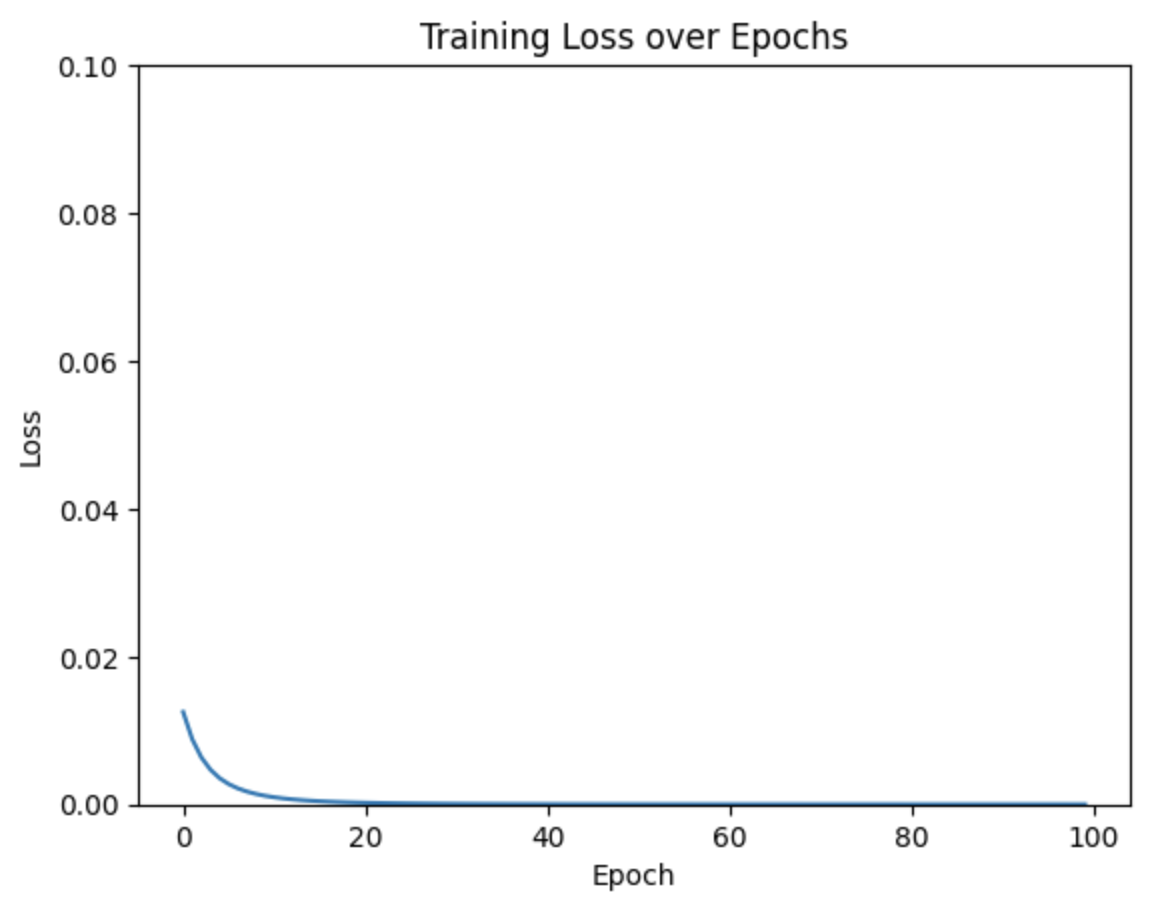
\includegraphics[width=0.5\linewidth]{Screenshot 2024-04-12 at 12.24.09 PM.png}
        \caption{Single Layer FNN}
        \label{fig:enter-label}
    \end{figure}
    \begin{figure}
        \centering
        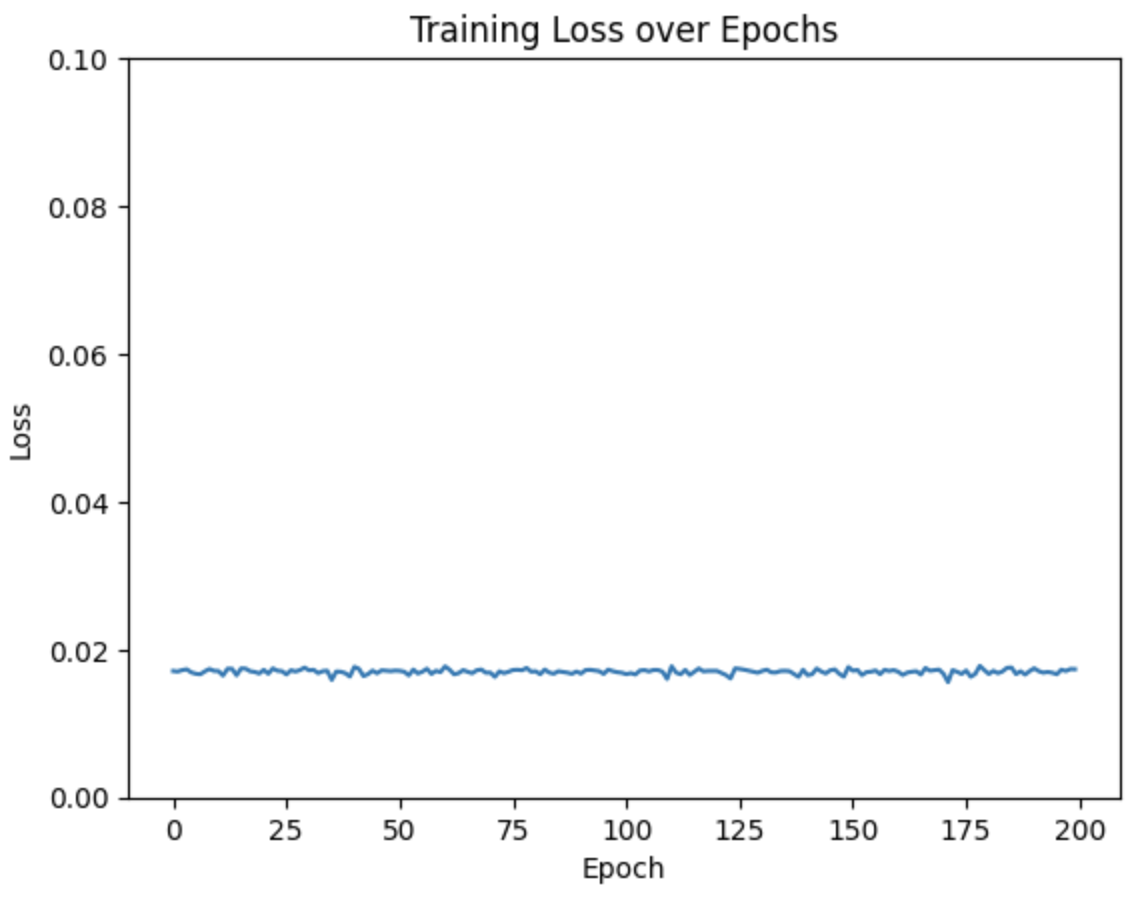
\includegraphics[width=0.5\linewidth]{Screenshot 2024-04-12 at 12.23.47 AM.png}
        \caption{Multilayer Layer FNN w/ lr 0.2}
        \label{fig:enter-label}
    \end{figure}
    \begin{figure}
        \centering
        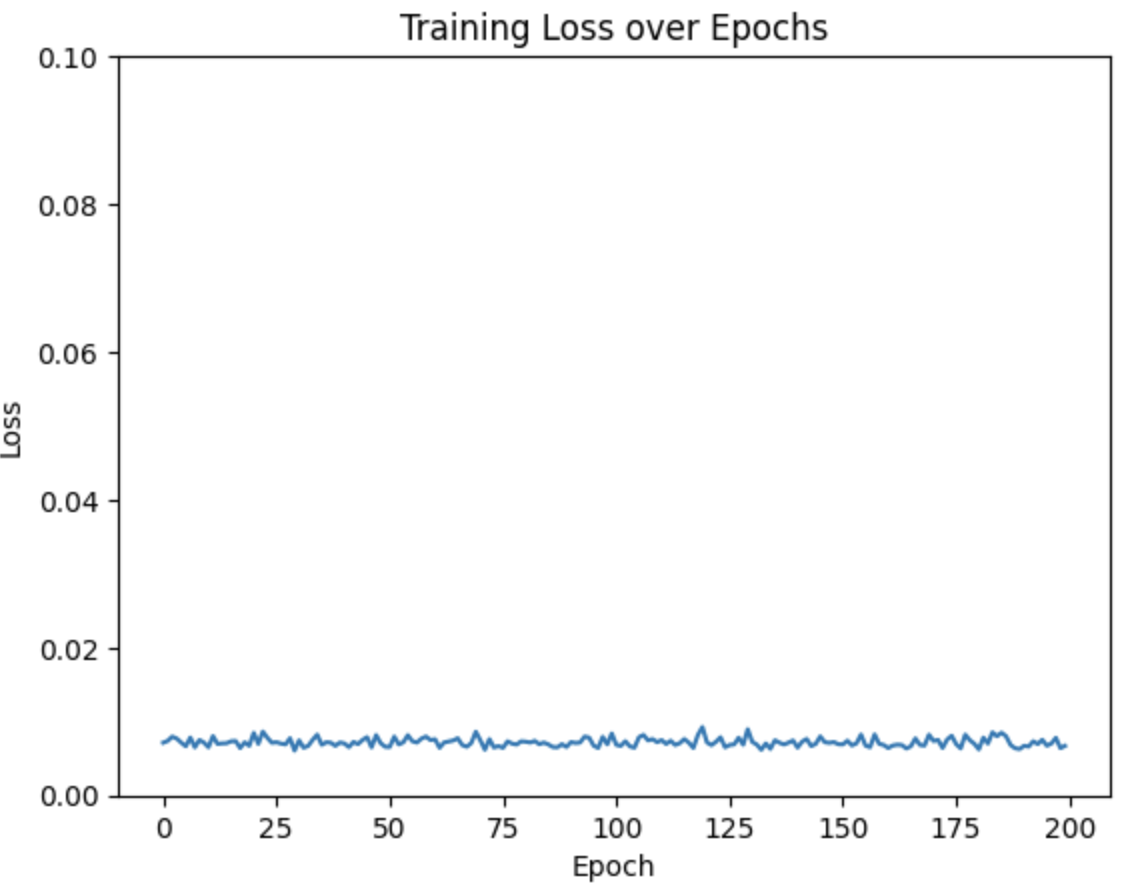
\includegraphics[width=0.5\linewidth]{Screenshot 2024-04-12 at 12.23.05 AM.png}
        \caption{Multilayer Layer FNN w/ lr 0.9}
        \label{fig:enter-label}
    \end{figure}
    \begin{figure}
        \centering
        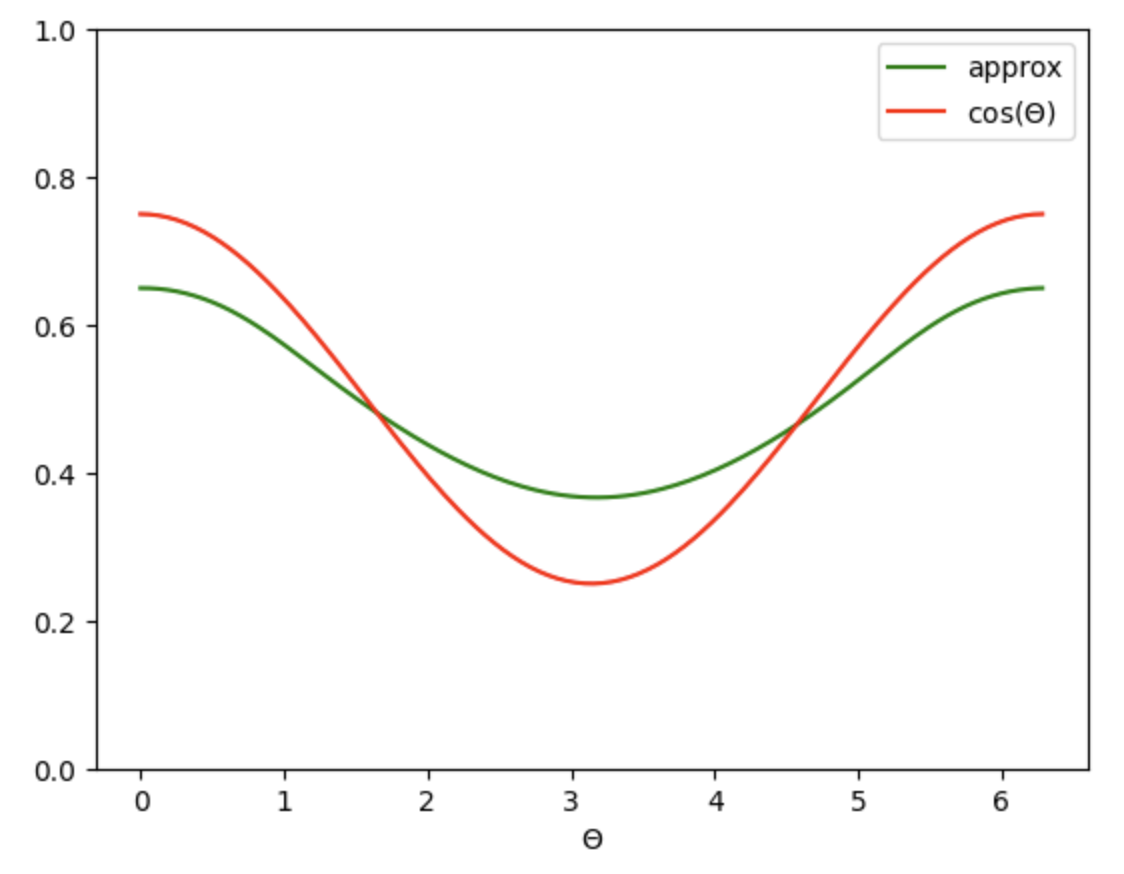
\includegraphics[width=0.5\linewidth]{20, 10 parameters.png}
        \caption{20 inputs, 10 hidden}
        \label{fig:enter-label}
    \end{figure}
    \begin{figure}
        \centering
        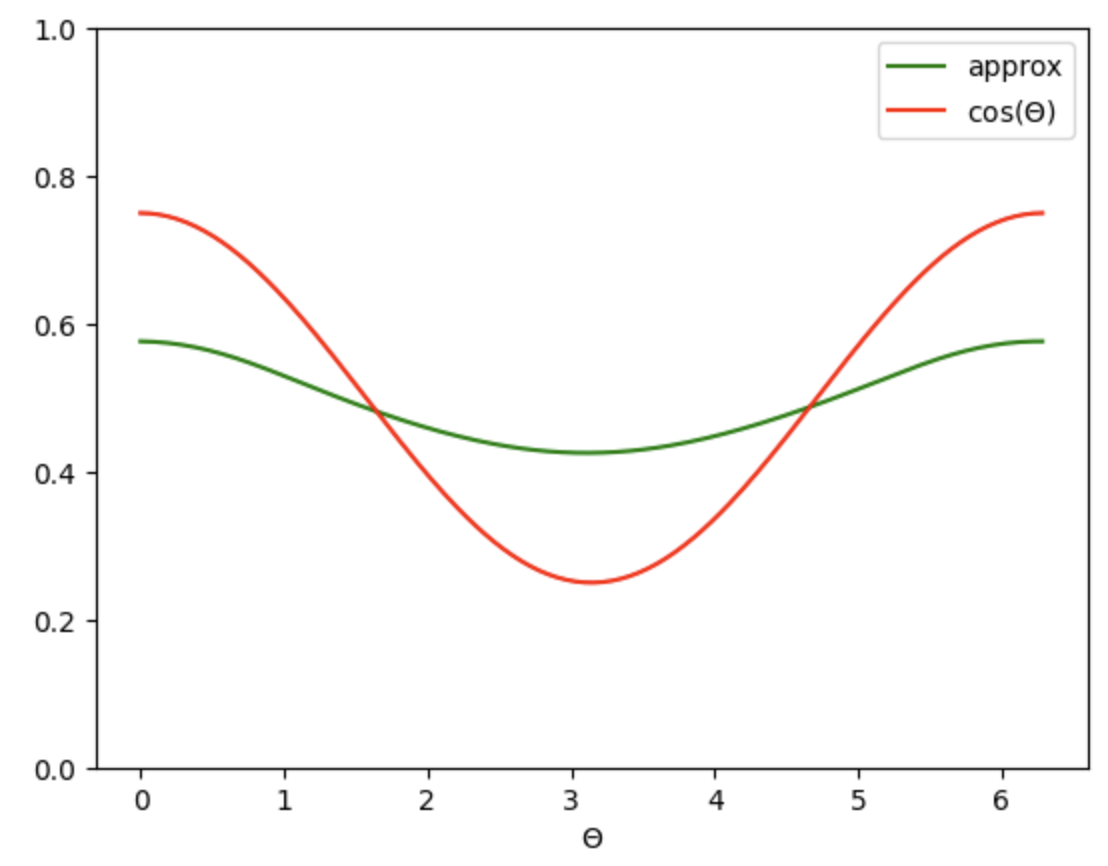
\includegraphics[width=0.5\linewidth]{50, 30 parameters.png}
        \caption{50 inputs, 30 hidden}
        \label{fig:enter-label}
    \end{figure}

\end{itemize}

\newpage

\end{document}